\documentclass[a4paper, 11pt]{article}
\usepackage{fullpage}
\usepackage{mathtools, nccmath}
\usepackage{graphicx}
\usepackage{float}
\usepackage{amsmath}
\renewcommand{\figurename}{Fig.}
\renewcommand{\refname}{Bibliografia}


\begin{document}
%Header
\noindent
\large\textbf{Corso di Metodi di Ottimizzazione} \hfill \textbf{Gruppo E} \\
\normalsize A.A. 2018/2019 \hfill Ing. Saverio Del Prete \\
Prof. Raffaele Martone \hfill Ing. Bernardo Giordano \\
\hphantom{}\hfill Ing. Lucia Migliaccio

\section*{Traccia del problema}

Progetto ottimo di un campo magnetico con incognite geometriche e di corrente di
una spira.

\section*{Descrizione del sistema fisico}

Il sistema è composto da un certo numero di spire simmetriche (supporremo $n=6$)
concentriche rispetto allo stesso asse $z$. I parametri di progetto, ovvero
posizione, raggio e intensità di corrente, sono noti per tutte le spire tranne
che per una coppia.

\begin{figure}[H]
	\centering
	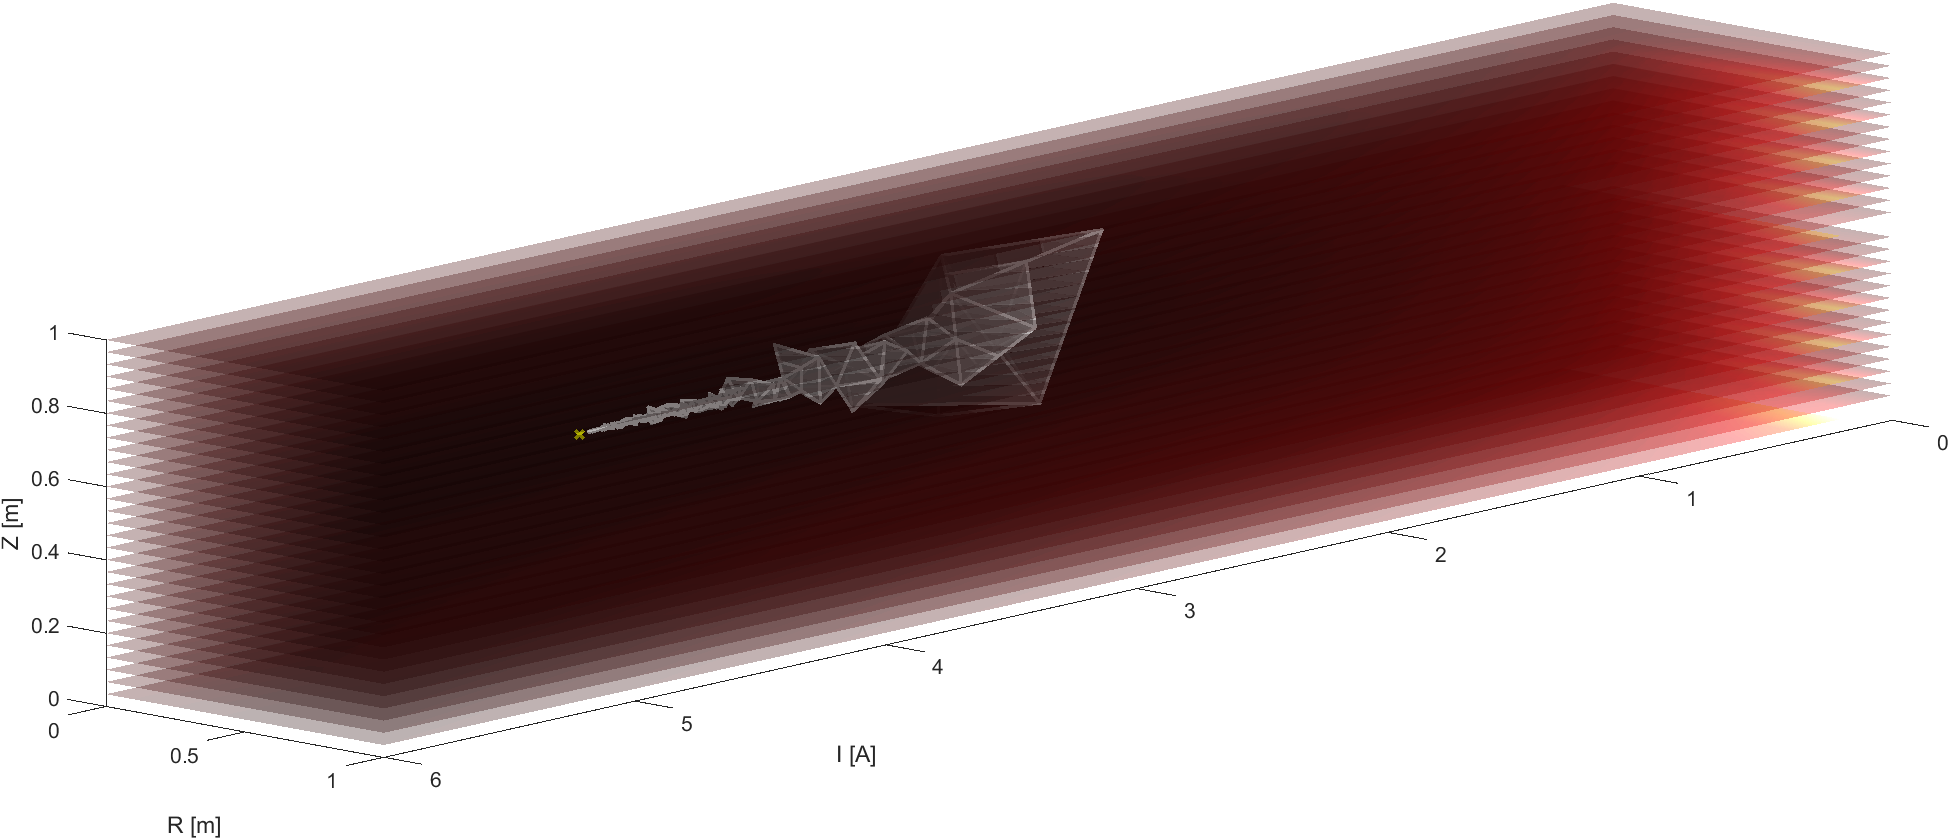
\includegraphics[width=12cm]{assets/figure4}
	\caption{Sistema fisico posizionato nel piano $xyz$.}
\end{figure}

\noindent
Il campo magnetico generato dalla corrente circolante nelle spire può essere
valutato sull’asse utilizzando la legge di Biot-Savart. La legge di Biot-Savart
ci permette di valutare il campo magnetico B prodotto in un punto dello spazio
da una spira percorsa da corrente elettrica.


\noindent
Il campo magnetico sull’asse $z$  di una spira caratterizzata da una corrente
$I$, lunghezza $L$, raggio $R$ e posizione $Z$ (supponiamo, per
semplicità, posizionata in $Z=0$), si valuta come
\[dB_{z}=\frac{\mu_{0}IdL}{4\pi}\frac{R}{\left(z^{2}+R^{2}\right)^{3/2}}\]
dove $\mu_{0}$ è la permeabilità magnetica nel vuoto, $\mu_{0}=4{\pi}10^{-7}
H/m$. \\
L’integrale di $dL$ risulta essere proprio la circonferenza della spira, ovvero
$2{\pi}R$. Integrando quindi, si ricava la funzione del campo magnetico
sull'asse
\[B_{z}=\frac{\mu_{0}}{4\pi}\frac{2{\pi}R^{2}I}{\left(z^{2}+R^{2}\right)^{3/2}}=\frac{\mu_{0}}{2}\frac{R^{2}I}{\left(z^{2}+R^{2}\right)^{3/2}}\]
Siano $Z_{i}$, $R_{i}$ e $I_{i}$ rispettivamente la posizione, il raggio e la
corrente relative alla spira $i$-esima. \\
Sia inoltre $n=6$ il numero complessivo delle spire facenti parte del sistema.
Considerando adesso la sovrapposizione degli effetti di tutte le spire del
sistema e tenendo presente che le spire sono simmetriche rispetto al piano $xy$,
il campo magnetico complessivo sull’asse $z$ sarà:

\begin{align*}
	B_{z}
	&=\frac{\mu_{0}}{4{\pi}}\left(\sum_{i=1}^{n/2}\frac{2{\pi}I_{i}R_{i}^{2}}{\left(\left(Z_{i}-z\right)^{2}+R_{i}^{2}\right)^{3/2}}+\frac{2{\pi}I_{i}R_{i}^{2}}{\left(\left(Z_{i}+z\right)^{2}+R_{i}^{2}\right)^{3/2}}\right)\\
	&=\frac{\mu_{0}}{2}\left(\sum_{i=1}^{n/2}\frac{I_{i}R_{i}^{2}}{\left(\left(Z_{i}-z\right)^{2}+R_{i}^{2}\right)^{3/2}}+\frac{I_{i}R_{i}^{2}}{\left(\left(Z_{i}+z\right)^{2}+R_{i}^{2}\right)^{3/2}}\right)
\end{align*}
\noindent
L'obiettivo del progetto della spira mancante risulta essere la migliore
approssimazione di un campo magnetico avente la seguente caratteristica:

\begin{figure}[H]
	\centering
	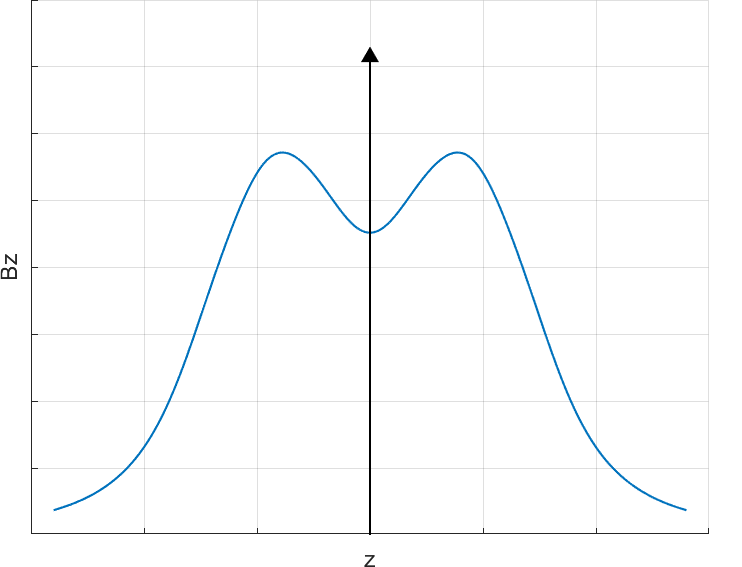
\includegraphics[width=10cm]{assets/figure3}
	\caption{Campo magnetico sull'asse $z$ desiderato.}
\end{figure}
\noindent
Sia adesso $B_{z}$ il campo magnetico generato dalla sovrapposizione delle spire
del sistema da progettare, e $\tilde{B_{z}}$ il campo magnetico desiderato. Al
fine da ottenere una discrepanza più piccola possibile, è di nostro interesse lo
studio della funzione
\[||B_{z}-\tilde{B_{z}}||\] dove $B_{z}$ è la funzione del campo magnetico da
progettare e $\tilde{B_{z}}$ è quella del campo desiderato. \\
Siccome i parametri di progetto delle spire 1 e 3 (e, quindi, delle rispettive
spire simmetriche) sono noti ed esattamente uguali a quelli del sistema
desiderato, la suddetta differenza in norma si scriverà come:

\begin{equation}
	\begin{split}
		||B_{z}-\tilde{B_{z}}||
		=& \Bigl|\Bigl|\frac{\mu_{0}}{2}(\frac{I_{2}R_{2}^{2}}{((Z_{2}-z)^{2}+R_{2}^{2})^{3/2}}+\frac{I_{2}R_{2}^{2}}{((Z_{2}+z)^{2}+R_{2}^{2})^{3/2}})- \\
		 & \frac{\mu_{0}}{2}(\frac{\tilde{I_{2}}\tilde{R_{2}}^{2}}{((\tilde{Z_{2}}-z)^{2}+\tilde{R_{2}}^{2})^{3/2}}+\frac{\tilde{I_{2}}\tilde{R_{2}}^{2}}{((\tilde{Z_{2}}+z)^{2}+\tilde{R_{2}}^{2})^{3/2}})\Bigr|\Bigr| \\
		=& \frac{\mu_{0}}{2}\Bigl|\Bigl|\frac{I_{2}R_{2}^{2}}{((Z_{2}-z)^{2}+R_{2}^{2})^{3/2}}+\frac{I_{2}R_{2}^{2}}{((Z_{2}+z)^{2}+R_{2}^{2})^{3/2}}- \\
		 & \frac{\tilde{I_{2}}\tilde{R_{2}}^{2}}{((\tilde{Z_{2}}-z)^{2}+\tilde{R_{2}}^{2})^{3/2}}+\frac{\tilde{I_{2}}\tilde{R_{2}}^{2}}{((\tilde{Z_{2}}+z)^{2}+\tilde{R_{2}}^{2})^{3/2}}\Bigr|\Bigr|
	\end{split} 
\end{equation}
\noindent


\section*{Analisi dei parametri}


Al fine di avvicinarci alla caratteristica descritta in $Fig.2$,
dobbiamo scegliere opportunamente il valore dei raggi, delle correnti e
delle posizioni relativi a tutte le spire, comprese quelle da progettare (spire
2 e 4). 
Dopo diverse iterazioni, vediamo che dei plausibili valori sono: 
\newline  \\
\centerline{ \textbf{Spira 1}: $R_{1}$ = 0.7m \\ $I_{1}$ = 3 A \\ $Z_{1}$ = -0.4m} 
\centerline{ \textbf{Spira 2}: $R_{2}$ = 0.8m \\ $I_{2}$ = 5 A \\ $Z_{2}$ = -0.7m}
\centerline{ \textbf{Spira 3}: $R_{3}$ = 0.6m \\ $I_{3}$ = 2 A \\ $Z_{3}$ = -0.9m}
\centerline{ \textbf{Spira 4}: $R_{4}$ = 0.7m \\ $I_{4}$ = 3 A \\ $Z_{4}$ = 0.4m}
\centerline{ \textbf{Spira 5}: $R_{5}$ = 0.8m \\ $I_{5}$ = 5 A \\ $Z_{5}$ = 0.7m}
\centerline{ \textbf{Spira 6}: $R_{6}$ = 0.6m \\ $I_{6}$ = 2 A \\ $Z_{6}$ = 0.9m}


\section*{Campionamento e normalizzazione}

Prima di poter definire la nostra funzione obiettivo, c'è bisogno di applicare
due tecniche, ovvero: campionamento e normalizzazione.
Il campionamento è una tecnica che consiste nel discretizzare un segnale
continuo nel tempo. La normalizzazione è l'operazione la quale, dato un vettore,
lo porta ad avere una norma unitaria. \\
Campionando la (1) vediamo che: 


\begin{equation}
	\begin{split}
		F_{obj} = 
		& \frac{\mu_{0}}{2} \frac{1}{Np} \sum\limits_{k=1}^{Np} \Biggl[\Bigl|\Bigl|\frac{I_{2}R_{2}^{2}}{((Z_{2}-z)^{2}+R_{2}^{2})^{3/2}}+\frac{I_{2}R_{2}^{2}}{((Z_{2}+z)^{2}+R_{2}^{2})^{3/2}}- \\
		& \frac{\tilde{I_{2}}\tilde{R_{2}}^{2}}{((\tilde{Z_{2}}-z)^{2}+\tilde{R_{2}}^{2})^{3/2}}+\frac{\tilde{I_{2}}\tilde{R_{2}}^{2}}{((\tilde{Z_{2}}+z)^{2}+\tilde{R_{2}}^{2})^{3/2}}\Bigr|\Bigr|\Biggr]
	\end{split} 
\end{equation}
\noindent
$N_{p}$ è il numero di campioni che andiamo a considerare. Essendo che, più
cresce il campionamento e più cresce la somma delle variabili andiamo a
valutarne la media. Infine, eseguiamo una normalizzazione del
campionamento rispetto alla media di $\tilde{B_{z}}$. La $funzione$ $obiettivo$ si
scriverà come:
 

\begin{equation}
	\begin{split}
		F_{obj} =
		& \frac{\mu_{0}}{2} \frac{1}{{\tiny <} \tilde{B_{z}}{\tiny >}} \Biggl\{ \frac{1}{Np} \sum\limits_{k=1}^{Np} \Biggl[\Bigl|\Bigl|\frac{I_{2}R_{2}^{2}}{((Z_{2}-z)^{2}+R_{2}^{2})^{3/2}}+\frac{I_{2}R_{2}^{2}}{((Z_{2}+z)^{2}+R_{2}^{2})^{3/2}}- \\
		& \frac{\tilde{I_{2}}\tilde{R_{2}}^{2}}{((\tilde{Z_{2}}-z)^{2}+\tilde{R_{2}}^{2})^{3/2}}+\frac{\tilde{I_{2}}\tilde{R_{2}}^{2}}{((\tilde{Z_{2}}+z)^{2}+\tilde{R_{2}}^{2})^{3/2}}\Bigr|\Bigr|\Biggr]\biggr\}^{\!1/2}
	\end{split} 
\end{equation}
\noindent
 

\section* {Ricerca del minimo}

L'algoritmo di ricerca del minimo fa uso del concetto di simplesso, cioè un politopo di N+1 vertici 
in N dimensioni, vale a dire: un segmento in una dimensione, un triangolo in due 
dimensioni, un tetraedro in tre dimensioni. Il metodo ci permette di limitare la
ricerca della soluzione ottima ai vertici del politopo. La ricerca avviene 
attraverso il movimento del politopo, il quale può:\\   
-Ribaltarsi:    valuto il valore della funzione nei 3 vertici, individuo il vertice
con il valore 'peggiore', ribalto rispetto a quest'ultimo tenendo fermo gli
altri due vertici(caso N=2). L'algoritmo può trovarsi in una
	condizione di loop, questo avviene quando il valore della funzione nel vertice ribaltato, continua ad
	essere il peggiore. In questo caso particolare, si applica il metodo
	del "secondo peggiore", ossia, si torna al passo precedente e si va a
	valutare il vertice con il secondo valore peggiore e si procede con il
	ribaltamento. \\
-Contrarsi:     se un vertice del politopo rimane più a lungo di un numero 
	specifico di iterazioni M (M fissato) il politopo viene contratto.\\
Il simplesso è un metodo zero-th, anche se non faccio uso di derivate sto stimando in qualche
modo una direzione di discesa. \\

\section* {Esperimenti con il metodo del simplesso}
L'algoritmo del simplesso è stato implementato su matlab, ma prima di
considerare il problema vero e proprio, si è ritenuto opportuno effetturare diversi esperimenti.
Partiamo col dire che, nel nostro caso, avendo tre incognite: la corrente $I_{2}$, il raggio $R_{2}$ e
la posizione $Z_{2}$, avremo come politopo un tetraedro.\\

%Il primo esperimento è stato fatto in 2d senza applicare alcun vincolo. 
%dati e figura 2d
%In seguito è stato fatto l'esperimento in 3d, con le stesse modalità.
%dati e figura 3d 

\begin{thebibliography}{9}
	% \bibitem{id}Author\emph{title}[online]. Editor.
\end{thebibliography}
\end{document}